\documentclass[12pt]{report}
\usepackage{amsmath}
\usepackage{amssymb}
%\usepackage{keyval}
\usepackage{graphicx}
\usepackage{tikz}

\newcommand{\bt}[1]{\textbf{#1}}
\newcommand{\ubt}[1]{\textbf{\underline{#1}}}
\newcommand{\sps}{\\[0.2cm]}
\newcommand{\spn}[1]{\\[#1cm]}
\newcommand{\refn}[1]{\textbf{(\ref{#1})}}
\newcommand{\NI}{\noindent}
\newcommand{\beq}{\NI$\displaystyle}
\newcommand{\eeq}{$}
\newcommand{\eeqn}{$\\[0.3cm]}
\newcommand{\dsp}{\displaystyle}

\renewcommand*\contentsname{Table of Contents}
\renewcommand{\baselinestretch}{1.5}

\begin{document}
	
	\clearpage
	\thispagestyle{empty}
	%%TITLE%%
	\addcontentsline{toc}{chapter}{\numberline{}Title Page}
	\begin{center}
		{\bf GENDER INEQUALITY OF CONSTRUCTION WORKERS IN TIRU CHAPPALLI(TRICHY) }
	\end{center}
	$$$$
	\begin{center}
		\textbf{\itshape\large BY}
	\end{center} 
	$$$$
	\begin{center}
		{\bf ABDULKAREEM, LAWAL BABAITA\\
			16/30GP002}
	\end{center}
	$$$$
	\begin{center}
		\textbf{A PROJECT SUBMITTED TO THE
			DEPARTMENT OF MATHEMATICS, FACULTY OF PHYSICAL SCIENCES,
			UNIVERSITY OF ILORIN, ILORIN, NIGERIA,
			$$$$
			IN PARTIAL 
			FULFILLMENT OF REQUIREMENTS FOR THE AWARD OF
			BACHELOR OF SCIENCE {\itshape{(B.Sc.)}} DEGREE IN MATHEMATICS.}
	\end{center}
	$$ $$ 
	\\ \\
	\begin{center}
		{\bf 	April, 2021}
	\end{center}
	%%%%Certification
	\newpage
	\pagenumbering{roman} 
	\addcontentsline{toc}{chapter}{\numberline{}Certification}
	\section*{\begin{center}\textbf{\Large Certification}   \end{center}}
	This is to certify that this project was carried out by \textbf{ABDULKAREEM, LAWAL BABAITA} of Matriculation Number  16/30GP002, for the award of Bachelor of Science B.Sc (Hons) degree in the Department of Mathematics, Faculty of Physical sciences, University of Ilorin, Ilorin, Nigeria.
	\\
	\\
	................................... \qquad \qquad\qquad\qquad\qquad\qquad...................... \\
	PROF. K. RAUF   \qquad\qquad\qquad\qquad\qquad\qquad\qquad\quad Date\\
	(SUPERVISOR)\\
	\\
	\\
	\\
	...................................... \qquad\qquad\qquad\qquad\qquad\qquad ......................\\
	PROF. K. RAUF      \qquad\qquad\qquad\qquad\qquad\qquad\qquad\qquad    Date\\
	(HEAD OF DEPARTMENT)\\
	\\
	\\
	\\
	..................................... \qquad\qquad\qquad\qquad\qquad\qquad .......................\\
	EXTERNAL EXAMINER \qquad\qquad\qquad\qquad\qquad\qquad         Date\\
	
	\newpage
	%%DEDICATION%%
	\section*{\begin{center}	\textbf{\Large Dedication}   \end{center}}
	\addcontentsline{toc}{chapter}{\numberline{}Dedication}
	
	First 
	
	\newpage
	%%ACKNOLEDGEMENT%%
	\section*{\begin{center}\textbf{\Large Acknowledgments}\end{center}}
	\addcontentsline{toc}{chapter}{\numberline{}Acknowledgments}
	I gave all glory, honour and 
	
	\newpage
	%%ABSTRACT%%
	\section*{\begin{center}\textbf{\Large Abstract}\end{center}}
		\addcontentsline{toc}{chapter}{\numberline{}Abstract}
		In
		
	%%TABLE OF CONTENTS%%
	\addcontentsline{toc}{chapter}{\numberline{}Table of Contents}
	\tableofcontents
	\newpage
	
	\pagenumbering{arabic}
	%%%%%%%%%%%%%%%%%%%%%%%%%CHAPTER ONE%%%%%%%%%%%%%%%%%%%%%%%%%%%%
	\chapter{}
	\section{INTRODUCTION TO INEQUALITIES}
	Mathematicians as well as Mathematics educators can attest to the importance of inequalities not only in the study of Mathematics but also n the normal life activities.
	
	Consider building blocks for many Mathematical areas, inequalities are studied for three particular reasons, which are as follows;
	\begin{itemize}
		\item Practical
		\item Theoretical and
		\item Aesthetic
	\end{itemize}

	\subsection{PRACTICAL}
	At the practical level, from the early involvement with problem solving, one must learn to build variables or learn to write restrictions for the unknowns, and these are expressed as inequalities.
	
	\subsection{THEORETICAL}
	Theoretically, inequalities used to express the domain of a function to prove limits, to setup research questions that relate equations to special cases that are inequalities or to prove equality by means of inequalities.\spn{-.3}
	
	\NI Moreover, Mathematicians testify that there are many aesthetic aspects in inequalities as well as in some of their proofs.
	
	\subsection{AESTHETIC}
	Aesthetic in Mathematics encompasses an appreciation of the beauty elegance and significance of Mathematical entities. A generation of hormonions and permanent patterns, a perseverance in continuing a journey even when one is lost in misleading positions. All these aspects are present in the work of a Mathematicians concerned with inequalities.
	
	
	\section{DEFINITION OF INEQUALITIES}
	\begin{description}
		\item[DEF 1.1] Inequalities is comparison of two values or expressions. An inequalities compares two statements with different values.
		\item[DEF 1.2] In Mathematics, Inequalities is a relationship between two different quantities or values.
	\end{description}
	Inequalities is a Mathematical expression that one quantity is greater than or less than another quantity.
	
	\NI\bt{For Example}\\
	"a\bt{ is less than } b"\spn{-.4}
	
	\NI \bt{NOTE:} The above expression can be written symbolically\\
	$\displaystyle a < b$ [i.e the left hand side is lower than \{ i.e less than\} the right hand side]\spn{-0.3}
	
	\NI Also,\\
	"a \bt{is greater than } b"\\
	It can also be written symbolically as,\\
	$\displaystyle a > b$ [i.e the left hand side is greater than \{ i.e higher than\} the right hand side]\spn{-0.3}
	
	\NI The above expressions are examples of inequalities.\\
	
	\NI Also, the express $x$ greater than 10 \{i.e symbolically $x > 10$ \} is an inequality, whereas, $x$ equal to 10 \{ i.e symbolically $x = 10$ \} is an equation.\\
	
	\NI Recall that an equation is a statement declaring the equality of two expressions.
	
	\NI For example; $5x + 5 = 3$ is an equation\spn{-.5}
	
	\NI And inequality compares two statements with different values. Example $5x + 5 \leq 30$ is an inequality.
	
	\section{THE USE OF SYMBOLS IN INEQUALITIES}
	
	The use of symbols make inequalities expression in Mathematics more easier to express.\spn{-.3}
	
	\NI The inequality expression "a is less than b" is easily denoted by "$a < b$", also the inequality expression "a is greater than b" is easily denoted by "$a > b$".\spn{-.4}
	
	\NI Also, we can also have the inequality expression "a is greater than or equal to b" and "a is less than or equal to b" which is also symbolically denoted by "$a \geq b$" and "$a \leq b$" respectively.\spn{-.3}
	
	\NI Therefore, we can easily say inequalities is defined whenever we have two expressions linked with one of the following five(5) symbols
	\begin{enumerate}
		\item $<$ \quad ---\quad less than \{the left hand side is less than the right hand side\}
		
		\item $>$ \quad ---\quad greater than \{the left hand side is greater than the right hand side \}
		
		\item $\leq$ \quad ---\quad less than or equal to \{the left hand side is less than or equal to the right hand side \}
		
		\item $\geq$ \quad ---\quad greater than or equal to \{the left hand side is greater than or equal to the right hand side\}
		
		\item $\neq$ \quad ---\quad not equal to \{the left hand side is not equal to the right hand side\}
	\end{enumerate}
	\section{RULES FOR INEQUALITIES}
	\begin{enumerate}
		\item $A\leq B \implies A + C \leq B + C$
		\item $A \leq B \implies A - C \leq B - C$
		\item if $C > 0$, then $A \leq B \implies CA \leq CB$
		\item if $C < 0$, then $A \leq B \implies CA \geq CB$
		\item if $A > 0$ and $B > 0$, then $A \leq B \implies \frac{1}{A} \geq \frac{1}{B}$
		\item if $A \leq B$ and $C \leq D$, then $A + C \leq B + D$
	\end{enumerate}
	
	\section{NOTATIONS IN INEQUALITIES}
	\begin{enumerate}
		\item $a<b$ (means $a$ is smaller than $b$)
		\item $a>b$ (means $a$ is greater than $b$)
		\item $a \leq b$ (means $a$ is smaller/less than or equal to $b$)
		\item $a \geq b$ (means $a$ is greater than or equal to $b$)
		\item $a \neq b$ (means $a$ is not equal to $b$)
	\end{enumerate}
		
	\section{TYPES OF INEQUALITIES}
	\begin{enumerate}
		\item LINEAR INEQUALITIES
		\item QUADRATIC INEQUALITIES
		\item COMPOUND INEQUALITIES
		\item ABSOLUTE VALUE INEQUALITIES
	\end{enumerate}
		
	\subsection{LINEAR INEQUALITIES}
	A Linear inequality is an inequality which involves a linear function. A linear inequality looks exactly like a linear equation with the inequality sign replacing the equality sign.\\
		
	\NI \ubt{Examples of Linear Inequalities}
	\begin{enumerate}
		\item $x^2 + 5x \leq 22$ (i.e $x^2 + 5x$ is less than or equal to 22)
			
		\item $5x + 7 < 7$ (i.e $5x + 7$ is less than 7)
			
		\item $7y^2 - 4 \geq 6$ (i.e $7y^2 - 4$ is greater than or equal to 6)
			
		\item $4x + 14 > 10$ (i.e $4x + 14$ is greater than 10)
			
		\item $2x^3 - 4 \neq 5$ (i.e $2x^3 - 4$ is not equal to 5)
	\end{enumerate}
	
	\subsection{QUADRATIC INEQUALITIES}
	A quadratic inequalities is a function whose degree is 2 and where the $y$ is not always exactly equal to the function. These types of functions use symbols called inequality symbols that include the symbols we known \bt{"less than, greater than, less than or equal to and greater than or equal to}. So instead of seeing an equal sign, you will see these inequality symbols.\\
		
	\NI All quadratic inequalities are of the form $\mathbf{ax^2 + bx + c}$, where $\mathbf{a}$, $\mathbf{b}$ and $\mathbf{c}$ are numbers. The numbers $\mathbf{b}$ and $\mathbf{c}$ can be $\mathbf{0}$, but $\mathbf{a}$ must be equal to a number. It cannot be $\mathbf{0}$. This is because our quadratic inequality must have an $\mathbf{x^2}$ value. The other two terms do not need to be there.\\
		
	\NI\ubt{Examples}
	\begin{enumerate}
		\item $x^2 + 5x \leq 10$ (i.e $x^2 + 5x$ is less than or equal to 10)
			
		\item $x^2 + 2x \geq 5$ (i.e $x^2 + 2x$ is greater than or equal to 5)
	\end{enumerate}
	
	\subsection{COMPOUND INEQUALITIES}
	A compound inequalities is an equation with two or more inequalities joined together with either \bt{"and"} or \bt{"Or"}\\
		
	\NI\ubt{Examples}
	\begin{enumerate}
		\item $x \geq b$ and $x < 3$
		\item $x < -12$ or $x \geq 8$
	\end{enumerate}
		
	When two inequalities are joined with \bt{"and"}, they are often written simply as a double inequality, for example $-6 \leq x < 3$. The solution of an \bt{"and"} in inequalities is the intersection of each individual inequality in the sentence.
		
	\subsection{ABSOLUTE VALUE INEQUALITIES}
	Let first return to the original definition of absolute value;\\
	
	\NI Absolute Value $(x)$ is the distance of $x$ from zero. For instance, both $-2$ and $+2$ are two units from zero, as it is shown in the image below\\
		
	\begin{center}
		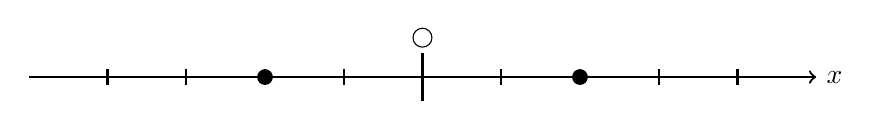
\begin{tikzpicture}
			\draw[thick, ->] (-1,0) -- (9,0) node[right]{$x$};
			\foreach \x in {0,1,...,8}
				\draw[thick] (\x,0.1) -- (\x,-0.1);
			\draw[thick] (4,.3) -- (4,-.3);
			\draw (4,.5) circle(1.2mm);
			\fill (2,0) circle(1mm);
			\fill (6,0) circle(1mm);
		\end{tikzpicture}
	\end{center}
		
	\NI This means that these absolute values will both be 2: that is, we have $|-2| = |+2| = 2$\\
	
	\NI With this definition and image in mind, let's now define Absolute Value Inequalities.\spn{-.5}
		
	\NI\bt{Absolute Value Inequality is an inequality that has an absolute value sign with a variable inside.}\spn{-.4}
		
	\NI\ubt{Examples}\\
	$|x| < 4$ (means that the distance between $x$ and $0$ is less than $4$)\\
	$|x| > 3$ (means that the distance between $x$ and $0$ is greater than $3$)\\
		
	\subsubsection{PROPERTIES OF AN ABSOLUTE VALUE INEQUALITIES}
	\begin{enumerate}
		\item $|x| < C \implies -C < x < C$ (i.e the distance between $0$ and $x$ is less than $C$)
			
		\item $|x| \leq C \implies -C \leq x \leq C$ (i.e the distance between $0$ and $x$ is less than or equal to $C$)
			
		\item $|x| > C \implies -C > x > C$ (i.e the distance between $0$ and $x$ is greater than $C$)
			
		\item $|x| \geq C \implies -C \geq x \geq C$ (i.e the distance between $0$ and $x$ is greater than or equal to $C$)
	\end{enumerate}
	
	\section{EXAMPLES OF INEQUALITIES IN DAILY LIFE}
	\NI(1) If Ade has N100 and wants to buy some biros and pencils, how many biros and pencils can he buy? Using inequality expression, write this statement Mathematically.\spn{-.6}
		
	\NI\ubt{Solution}\\
	Let number of biros be $x$\\
	and let number of pencils be $y$\\
	Amount owned by Ade $= \text{N}100$\\
	Therefore; $x + y \leq 100$\\
		
	\NI(2) Ibrahim receives N200 daily for his daily needs if he need to buys some books and bottle of water, how many books and bottle of water can he buy using inequality expression, thus, write this statement Mathematically\spn{-.6}
		
	\NI\ubt{Solution}\\
	Amount owned by Ibrahim $=\text{N}200$\\
	Let number of books bought be $=a$\\
	and let number of bottle of water bought be $=b$\\
	Therefore, $200 \geq a+b$\\
		
	\NI(3) Ola is a father of three children (Ade, Ope, and Tade). If the ages of the three children is added together and subtracted from Ola's age. How old is Ola. Use the inequality expression and write this statement Mathematically.\spn{-.6}
		
	\NI\ubt{Solution}\\
	Let Ola's age be $Q$\\
	Let the ages of Ola's children (Ade, Ope and Tade) be $x, y, z$ respectively,\\
	Therefore; $x + y + z \geq Q$\\
	
	
	
	%%%%%%%%%%%%%%%%%%%%%%%%%CHAPTER TWO%%%%%%%%%%%%%%%%%%%%%%%%%%%%
	\chapter{PROPERTIES OF INEQUALITIES}
	
	\subsubsection{(1) TRANSITIVE PROPERTY}
	The transitive property of inequality state that, for any real number $a,b,c,$
	\begin{enumerate}
		\item if $a > b$ and $b>c$, then $a > c$ (if $a$ is greater than $b$ and $b$ is greater than $c$, then $a$ is greater than $c$)
		
		\item if $a>b$ and $b \geq c$, then $a>c$ (if $a$ is greater than $b$ and $b$ is greater than or equal to $c$, then $a$ is greater than $c$)
		
		\item if $a < b$ and $b<c$, then $a<c$ (if $a$ is less than $b$ and $b$ is less than $c$, then $a$ is less than $c$)
	\end{enumerate}
	\newpage
	\ubt{Example}\\
	(1)If Ola is older than Ore and Ope is older than Tola, then Ola is older than Tola\\
	(2) If Tola has 4 mangoes and Ope has 3 mangoes, but Ola has 1 mango,\\
	Let represent mangoes owned by Tola to be $X$\\
	Let represent mangoes owned by Ope to be $Y$\\
	and, let represent mangoes owned by Ola to be $Z$\\
	then, $X>Y, \quad Y>Z, \text{ then } X >Z$\\
	
	\subsubsection{(2) REVERSAL PROPERTY}
	The Reversal property of inequality states that; for any real value $a$ and $b$,\\
	(1) if $a$ is greater than $b$, the $b$ is less than $a$. i.e if $a>b$, then $b<a$\\
	\ubt{Example}\\
	If Ola is older than Ope, then Ope is younger than Ola.
	
	\subsubsection{(3) LAW OF TRICHOTOMY}
	The law of trichotomy states that only one of the following is true: $a<b$, or $a=b$, or $a>b$\\
	
	\NI\ubt{Example}\\
	If Ola has more money than Ope, then we could write it like $a>b$ (representing Ola and Ope with $a$ and $b$ respectively)\\
	Also, we know that\\
	
	\NI Ola does not have less money than Ope (Not $a<b$)\\
	And, Ola does not have equal or the same money as Ope (Not $a \neq b$)
	
	\subsubsection{(4) SQUARE ROOT PROPERTY}
	It says taking a square root will not change the inequality but only when both $a$ and $b$ are greater than or equal to zero. That is, if $a<b$ then $\sqrt{a} \leq \sqrt{b}$ (for $a,b\geq 0$)\\
	
	\NI The above expression means if $a$ is less than or equal to $b$, then $\sqrt{a}$ is less than or equal to $\sqrt{b}$, if $a$, $b$ is greater than or equal to zero.\\
	
	\NI\ubt{Example}\\
	Let $a=4$\quad and\quad $b=25$\\
	So, if $a\leq b$\quad is\quad $4\leq 25$\\
	then $\sqrt{a} \leq \sqrt{b}$\quad is\quad $\sqrt{4} \leq \sqrt{25}$ (for $a,b \geq0$)
	
	\subsubsection{(5) ADDITION AND SUBTRACTION}
	It says that a common constant $c$ may be added or subtracted from both side of an inequality.\\
	That is, if $a<b$, then $a+c < b + c$\\
	
	\NI Also, for any real numbers $a, b, c$
	\begin{enumerate}
		\item if $a\leq b$, then $a+c \leq b+c$ and $a-c \leq b-c$
		
		\item if $a\geq b$, then $a+c \geq b+c$ and $a-c \geq b-c$
	\end{enumerate}
	
	\subsubsection{(6) ADDITIVE INVERSE}
	The Additive Inverse property states that; for any real numbers $a$ and $b$, negation will invert the inequality use
	\begin{enumerate}
		\item if $a \leq b$, then $-a \geq -b$
		
		\item if $a>b$, then $-a < -b$
	\end{enumerate}
	
	\NI As we just away, putting minuses(-) in from of real numbers $a$ and $b$ changes the direction of the inequality.\spn{0.3}
	This is called the Additive Inverse
	\begin{itemize}
		\item if $a<b$, then $-a > -b$
		\item if $a>b$, then $-a < -b$
	\end{itemize}
	
	\NI This is really the same as multiplying by (-1), and that is why it changes direction
	
	\subsubsection{(7) MULTIPLICATIVE INVERSE}
	The property for the multiplication inverse state that; for any non-zero real number $a$ and $b$, that are both positive or both negative, taking the reciprocal $\left(\text{i.e } \frac{1}{\text{value}}\right)$ of both $a$ and $b$ can change the direction of the inequality.\\
	
	\NI When $a$ and $b$ are both positive or both negative, i.e;
	\begin{itemize}
		\item if $a<b$ then $\frac{1}{a} > \frac{1}{b}$
		\item if $a>b$ then $\frac{1}{a} < \frac{1}{b}$
	\end{itemize}
	
	\NI These can also be written in chained notation as follows:\\
	for any non-zero real numbers $a$ and $b$;
	\begin{enumerate}
		\item if $0<a \leq b$, then $\frac{1}{a} \geq \frac{1}{b} > 0$
		\item if $a<b<0$, then $0 > \frac{1}{b} > \frac{1}{a}$
		\item if $a<0<b$, then $\frac{1}{a}<0<\frac{1}{b}$
		\item if $0\geq0>b$, then $\frac{1}{b} < \frac{1}{a} \leq 0$
		\item if $a>b>0$, then $0 < \frac{1}{b} < \frac{1}{a}$
	\end{enumerate}	
	
	\section{POWER INEQUALITIES}
	A Power Inequality is an inequality containing terms of the form $a^b$, where $a$ and $b$ are real positive numbers or variable expressions.\spn{0.4}
	\ubt{Examples}\\
	for any real number $x$,
	\begin{enumerate}
		\item $e^x \geq 1 + x$
		\item if $\displaystyle x>0$ and $p>0$, then \\ $\frac{x^p-1}{p} \geq \ln(x) \geq \frac{1-\frac{1}{x^p}}{p}$ \\
		
		\NI In the limit of $p\rightarrow 0$, then upper and lower bounds converge to $ln(x)$
		
		\item if $x>0$, then \\
		     $\displaystyle x^x \geq (\frac{1}{e})^{\frac{1}{e}}$
		
		\item $x \geq 1$, then\\
			$\dsp (x+y)^z + (x+z)^z + (y+z)^x > 2$
			
		\item for any real distinct numbers $a$ and $b$\\
			$\dsp \frac{e^b - e^a}{b-a} > e^{(a+b)/2}$
	\end{enumerate}
	
	\section{THE NUMBER LINE}
	a number line is a line with numbers on it i.e
	\begin{center}
		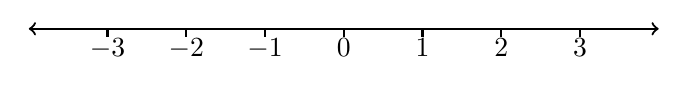
\begin{tikzpicture}
			\draw[thick, <->] (-4,0) -- (4,0);
			\foreach \x in {-3,-2,...,3}
			\draw[thick] (\x,-0.1)--(\x,0) node[below]{$\x$};
		\end{tikzpicture}
	\end{center}
	We use a number line to count and to graphically show numbers\\
	\ubt{Example}\\
	\begin{enumerate}
		\item Graph $x=5$ is expressed as\\
		\begin{center}
			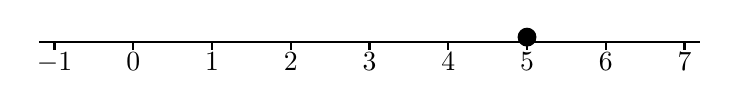
\begin{tikzpicture}
				\draw[thick] (-1.2,0) -- (7.2,0);
				\fill (5,0.06) circle(1.2mm);
				\foreach \x in {-1,0,...,7}
					\draw[thick] (\x,-0.1)--(\x,0) node[below]{$\x$};
			\end{tikzpicture}
		\end{center}
	
		\item Graph $x=-4$ is expressed as\\
		\begin{center}
			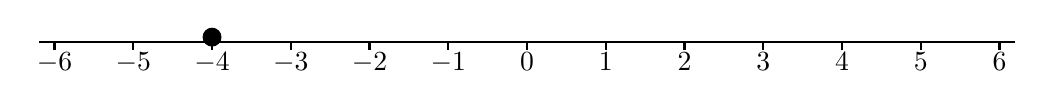
\begin{tikzpicture}
				\draw[thick] (-6.2,0) -- (6.2,0);
				\fill (-4,0.06) circle(1.2mm);
				\foreach \x in {-6,-5,...,6}
				\draw[thick] (\x,-0.1)--(\x,0) node[below]{$\x$};
			\end{tikzpicture}
		\end{center}
	\end{enumerate}
	\newpage
	\section{GRAPHING INEQUALITIES}
	Graph $x<3$
	\begin{center}
		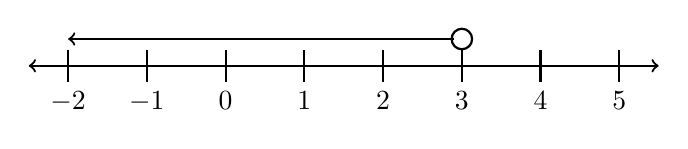
\begin{tikzpicture}
			\draw[thick, <->] (-2.5,0) -- (5.5,0);
			\draw[thick, <-] (-2,0.34) -- (2.9,0.34);
			\draw[thick] (3,0.34) circle(1.3mm);
			\foreach \x in {-2,-1,...,5}
				\draw[thick] (\x,0.2)--(\x,-0.2) node[below]{$\x$};
		\end{tikzpicture}
	\end{center}
	Also, Graph $x\leq3$
	\begin{center}
		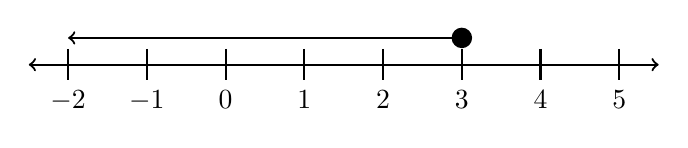
\begin{tikzpicture}
			\draw[thick, <->] (-2.5,0) -- (5.5,0);
			\draw[thick, <-] (-2,0.34) -- (2.9,0.34);
			\fill (3,0.34) circle(1.3mm);
			\foreach \x in {-2,-1,...,5}
			\draw[thick] (\x,0.2)--(\x,-0.2) node[below]{$\x$};
		\end{tikzpicture}
	\end{center}
	\bt{Note:}
	\begin{itemize}
		\item The solid shows that range of value that $x$ can take.
		\item The open circle on $3$ shows that although the solid line goes from 3, but $x$ cannot actually be equal to 3.
		\item The painted circle shows that $x$ can either be less than or equal to 3.
	\end{itemize}
	
	\NI\ubt{Examples}\\
	(1) Solve the inequality $4x + 6 > 3x + 7$ and represent the result on a number line\\
	\ubt{Solution}
	$4x + 6 > 3x + 7$\\
	firstly, we subtract 6 from both sides:\\
	we get; \quad $4x + 6-6 > 3x + 7 - 6$\\
	  $\left.\right.$\quad\qquad\quad= $4x > 3x + 1$\\
	Now, we subtract $3x$ from both sides\\
	We get, \quad $4x - 3x > 3x - 3x + 1$\\
	$\left.\right.$\quad\qquad\quad = $x > 1$\\
	representing $x>1$ on a number line\\
	\begin{center}
		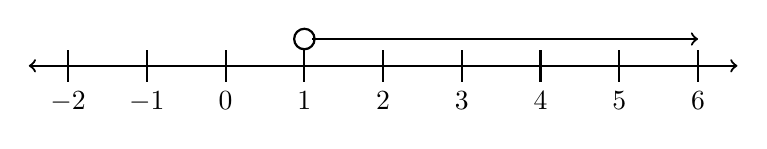
\begin{tikzpicture}
			\draw[thick, <->] (-2.5,0) -- (6.5,0);
			\draw[thick, ->] (1.1,0.34) -- (6,0.34);
			\draw[thick] (1,0.34) circle(1.3mm);
			\foreach \x in {-2,-1,...,6}
			\draw[thick] (\x,0.2)--(\x,-0.2) node[below]{$\x$};
		\end{tikzpicture}
	\end{center}

	\NI(2) For what values of $x$ are both the inequalities $9+2x >0$ and $7-3x>0$ are true?\\
	\ubt{Solution}\\
	if $9 + 2x>0$\\
	subtracting 9 from both sides,\\
	we get; \quad $9+2x-9>0-9$\\
	$\left.\right.\qquad\qquad 9-9 + 2x > 0-9$\\
	$\left.\right.\qquad\qquad = 2x > 0-9$\\
	$\left.\right.\qquad\qquad = 2x > -9$ 0r $\dsp x> -\frac{9}{2}$\\
	
	\NI Also, if $7-3x > 0$\\
	Subtracting $7$ from both sides\\
	We get; \quad $7-3x-7> 0 -7$\\
	$\left.\right.\qquad\qquad -3x > -7$ (negative cancels negative)\\
	$\left.\right.\qquad\qquad \implies 3x < 7$ or $\dsp x < \frac{7}{3}$\\
	
	\NI (Note: the reversed of the sign occurs when we divided both of the inequality by a negative numbers)\\
	We see that both sides inequalities are true for\\
	$$-\frac{9}{2} < x < \frac{7}{3}$$

	\NI representing the above inequality expression on a number line, we have;\\
	\begin{center}
		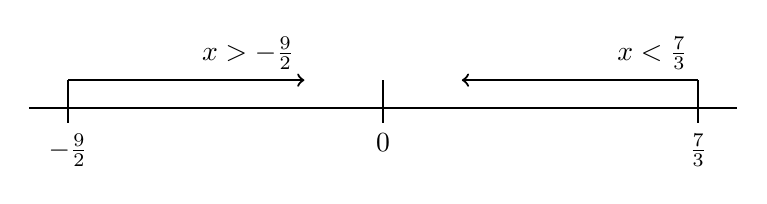
\begin{tikzpicture}
			\draw[thick] (-0.5,0)--(8.5,0);
			\draw[thick, ->] (0,0.35) -- (3,0.35) node[above left]{$x > -\frac{9}{2}$};
			\draw[thick, <-] (5,0.35) -- (8,0.35) node[above left]{$x < \frac{7}{3}$};
			\foreach \x /\y in{0/$-\frac{9}{2}$,4/0,8/$\frac{7}{3}$}
				\draw[thick] (\x,0.35)--(\x,-0.2) node[below]{\y};
		\end{tikzpicture}
	\end{center}
	
	\section{INEQUALITIES USED WITH A MODULUS SYMBOL}
	Inequalities often appear in conjunction with the modulus, or absolute value symbol $"|\;\;|"$ e.g $|x|<2$\\
	
	\NI Recall that the modulus of a number is simply its magnitude, or absolute value, regardless of its signs. So,\\
		$\left.\right.\qquad\qquad\qquad\qquad\qquad\qquad$ $|2|=2$ and $|-2|=2$\\
		
	\NI Now, $|x|<2$, it implies that $x$ must lies between 2 and -2, we can write it as $-2<x<2$, the range of value is shown in the number line, as shown below;
	\begin{center}
		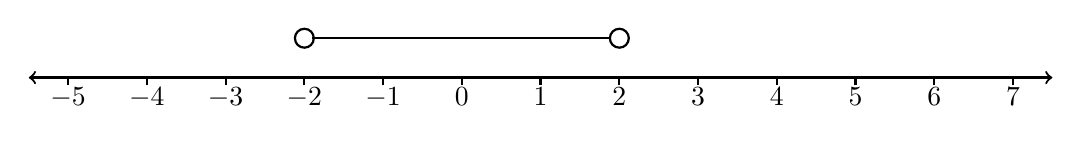
\begin{tikzpicture}
			\draw[thick, <->] (-5.5,0) -- (7.5,0);
			\draw[thick] (-2,0.5) circle(1.2mm);
			\draw[thick] (2,0.5) circle(1.2mm);
			\draw[thick] (-1.9,0.5) -- (1.9,0.5);
			\foreach \x in {-5,-4,...,7}
				\draw[thick] (\x,-0.1)--(\x,0) node[below]{$\x$};
		\end{tikzpicture}
		A number line showing $-2 < x < 2$\\
	\end{center}
	\ubt{Example}\\
	Suppose we want to solve the inequality $|x|\geq 5$\\
	
	\NI\ubt{Solution}\\
	If $|x| \geq 5$; This mean that the absolute value of $x$ must be greater than or equal to 5.\\
	
	\NI This also means that $x$ can be greater than or equal 5, or can be less than or equal to -5, we write $x\leq -5$ or $x\geq 5$. The range of values is shown below;
	\begin{center}
		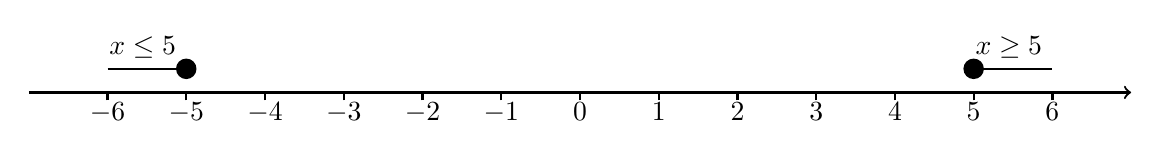
\begin{tikzpicture}
			\draw[thick,->](-7,0) -- (7,0);
			\draw[thick] (-6,0.3) -- (-5,0.3) node[above left]{$x\leq 5$};
			\draw[thick] (5,0.3) -- (6,0.3)node[above left]{$x\geq 5$};
			\fill (-5,0.3) circle(1.3mm);
			\fill (5,0.3) circle(1.3mm);
			\foreach \x in {-6,-5,...,6}
				\draw[thick] (\x,-0.1)--(\x,0) node[below]{$\x$};
		\end{tikzpicture}
		A number line showing $|x| \geq 5$\\
	\end{center}
	
	
	%%%%%%%%%%%%%%%%%%%%%%%%%CHAPTER THREE%%%%%%%%%%%%%%%%%%%%%%%%%%%%
	\chapter{METHODOLOGY}
	The aim of this study is to show through econometric analysis the presence of gender discrimination among construction workers and to test the hypotheses about which factors are contributing significantly to emergence of women as masons.\\
	
	\NI From this, we can generalize he finding obtained from the simple to the total study population. The study is micro in nature and data were collected from Trichy only. Every effort was taken to make sure that all the areas of Trichy were covered. Data regarding the number of construction workers in Trichy had to be forecasted.
	
	\section{AIM OF STUDY}
	The gender discrimination among construction workers and the ways to empower women construction workers in Tiruchirapalli is studied. Tiruchiraphalli, commonly known as Trichy is the fourth largest city of the Indian state of Tamil Nadu(after Chennai, Coimbatore and Madurai) and is also one of the A1 metropolitan cities of Tamil Madu. It is situated in the centre of the and on the banks of the River convery. Trichy is a corporation and the administrative headquarters of Tiruchisapalli District.
	
	\NI According to the 2001 census, Trichy or Tiruchirapalli had a population of 24,18,366. Males constitute 48.97 percent of the population and female 50.03 percent.\\
	
	\NI Trichy has an average literacy rate of 91.45 percent. Male literacy is 94.17 percent and female is 88.73 percent with 9.59 percent of the population under six years of age. Of the total female population, 16.7 percent are scheduled caste and of the total male population, 16.4 percent are scheduled caste. The total number of workers are 10,64,521, they constitute 6,87,814 male workers (64.6\%) and 3,76,707 female workers (35.4\%). Tamil is the official language.\\
	
	\NI The study was carried out for a period of four years, from October 2004 to September 2008. The data was collected in the year 2008.
	
	\section{DISTRIPTIVE STUDY}
	Distriptive studies involve describing the characteristics of a particular situation, event or case. This is a descriptive study as the problems faced by women construction workers and the reasons for women undertaking masonry work are determined. This study aims at describing and quantifying the distribution of certain variables in the study population at one point of time. They cover the following Socio-economic characteristics of men construction workers, the reasons for not involving women in masonry work, women construction workers willingness to be trained as masons and willingness to be become masons and willingness of men construction workers and contractors to train and accept masons are described.
	
	\section{TOTAL POPULATION OF CONSTRUCTION WORKERS IN TRICHY, TAMIL MADU}
	\ubt{Sampling Method}\\
	Various strategies can be used to collect quantitative data. However in the study stratified sampling was carried out. A sample of 440 women construction workers in Trichy was interviewed to find out their views on equal wages and motivation levels to be trained as women masons. A sample of 440 men construction workers in Trichy was interviewed to find out the suggestions for removing the gender disparity and women involving in masonry work. A sample of 51 contractors/Engineers in Trichy was asked to fill questionnaire to find out their views, ideas and suggestions on women in construction work. The construction workers were selected from "Santhai" (place where they are required for work), work places and wage disbursement centers.\\
	\ubt{Sampling Size}\\
	Sample size calculation (Krejcie and Morgan 1970)\\
	
	\begin{equation}
		\text{Sample Size }  = \frac{X^2 NP(1-P)}{d^2(N-1) + X^2P(1-P)} \tag{1}
	\end{equation}
	Where\\
	$\left.\right.$ \qquad\qquad $X^2=$ table value of Chi-Squared\\
	$\left.\right.$ \qquad\qquad d.f = 1 for desired confidence level (0.05 = 3.84)\\
	$\left.\right.$ \qquad\qquad $N=$ Total population size (42,422)\\
	$\left.\right.$ \qquad\qquad $P=$ Population proportion assumed to be 0.5\\
	$\left.\right.$ \qquad\qquad $d=$ degree of accuracy (expressed as a proportion) = 0.0327\\
	
	\NI Sample Size - 880 construction workers (440 women construction workers and 440 men construction workers) and 51 contractors\\
	
	\NI\ubt{Validity and Reliability}\\
	The content validity of the questionnaire was tested by a panel of experts. The validity of responses was tested using \bt{SPSS 15}. The reliability of the study was tested using Cronbach Coefficient Alpha. The Cronbach Coefficient Alpah is in a scale of 0 to +1. The higher the coefficient the better the measuring instrument. Cronbach's Alpha based on standardized items for the schedule for women workers is 0.668. Cronbach's Alpha for the schedule for men construction workers is 0.624. Cronbach's Alpha based on standardized items for the questionnaire for contractors is 0.648.\\
	
	\NI\ubt{Source of Data Collection}\\
	The method of data collection adopted for the study is primary. The primary data collected, is through interview schedule, which was collected from the Men and Women construction workers, the questionnaire was used to collect data from contractors in the study area (Appendix A,B, and C). As majority of the construction workers are illiterate, two schedules were prepared, one for women construction workers, and another for men construction workers and the construction workers interviewed in the local language (Tamil) and the responses were noted in the schedule.\\
	
	\NI The tools used for data collection is schedule and questionnaire. This was pre-tested by conducting a pilot study through which primary data was collected from 70 respondents. Analysis was done and changes were made in the schedule to overcome the errors. \\
	
	\NI In the schedule for women construction workers, question number 1-17 deal with socio-demographic factors of the respondents, question numbers 18-23 deal with the work remuneration, question numbers 24-28 deals with awareness of the respondents on unions, question number 29-42 deal with workplace condition and home background, question number 43-50 deal with bringing about an awareness in the women interviewed that they are also doing masonry job but are still paid lower and not allowed to take up the job of a mason, question number 51-53 deal with the reason for not doing masonry job and 54-57 deal with their willingness to be trained and to become Masons.\\
	
	\NI In the schedule for men construction workers, question number 1-19 deal with socio-demographic factors of the respondents, question numbers 20-25 deal with the work remuneration, question 26-30 deal with awareness of the respondents on unions, question numbers 31-43 deal with workplace conditions, question number 44 deals with the birnging about an awareness in the men interviewed that men are able to be promoted and take up masonry job as same as they learn the skill, question 45-47 deal with the reason for not doing masonry job and 48-58 deal with their willingness to train women as masons and to employ masons.\\
	
	\NI In the questionnaire for contractor, question numbers 1-10 deal with socio-demographic factors of the respondents, question numbers 11-14 deal with the work remuneration, question numbers 15-19 deal with unions, question numbers 20-22 deal with behaviour of women in workplace, questions number 23-26 deal with workplace conditions, question numbers 27-34 deal with workers attitude and number, questions numbers 35-38 deal in the reason for no women mason, 39-41 deal with their willingness to train women as masons to employ masons and finally questions 42 deals with the major problem that women construction workers face in the opinion of the contractor.\\
	
	\section{STATISTICAL TOOLS EMPLOYED}
	The Statistical tools employed are Econommetric analysis-t-test, On way ANOVA, Chi Square, Multiple Regression, Logistic Binary Regression and Charts.
	
	\section{SCOPE}
	This research is undertaken in Trichy, to remove gender discrimination in the construction industry in wages as women are paid less than men for the same job. There is a need to educate, train and motivate the women to take up the job as masons. There is also a need to educate the supervisors/contractors and other male masons to train and accept women masons and pay them equal salary like male masons and eradicate gender discrimination. This training of women masons can be done as experimental research.
	
	\section{LIMITATIONS}
	A pilot study was conducted and primary data were collected for 75 women construction workers. Analysis was done and certain difficulties were experience. However these were isolated and methods to overcome these hindrances were incorporated. The final data were collected from 440 men and 440 women construction workers and 51 contractors. The population of construction workers is scattered and coverage was a major problem.
	
	\section{CHAPTERISATION}
	The framework of the study is divided into six units in which the first unit which consists of the introduction. the second unit consists of the Review of Literature. The third unit discusses the objectives of the study, sampling design and scope of the study. The fourth unit consist fo data analysis and interpretation. The fifty unit consists of findings. The sixth unit consists of suggestions and conclusion.
	
\end{document}

